\begin{wrapfigure}[2]{r}[-1cm]{3cm}
 \vspace{-6cm}
  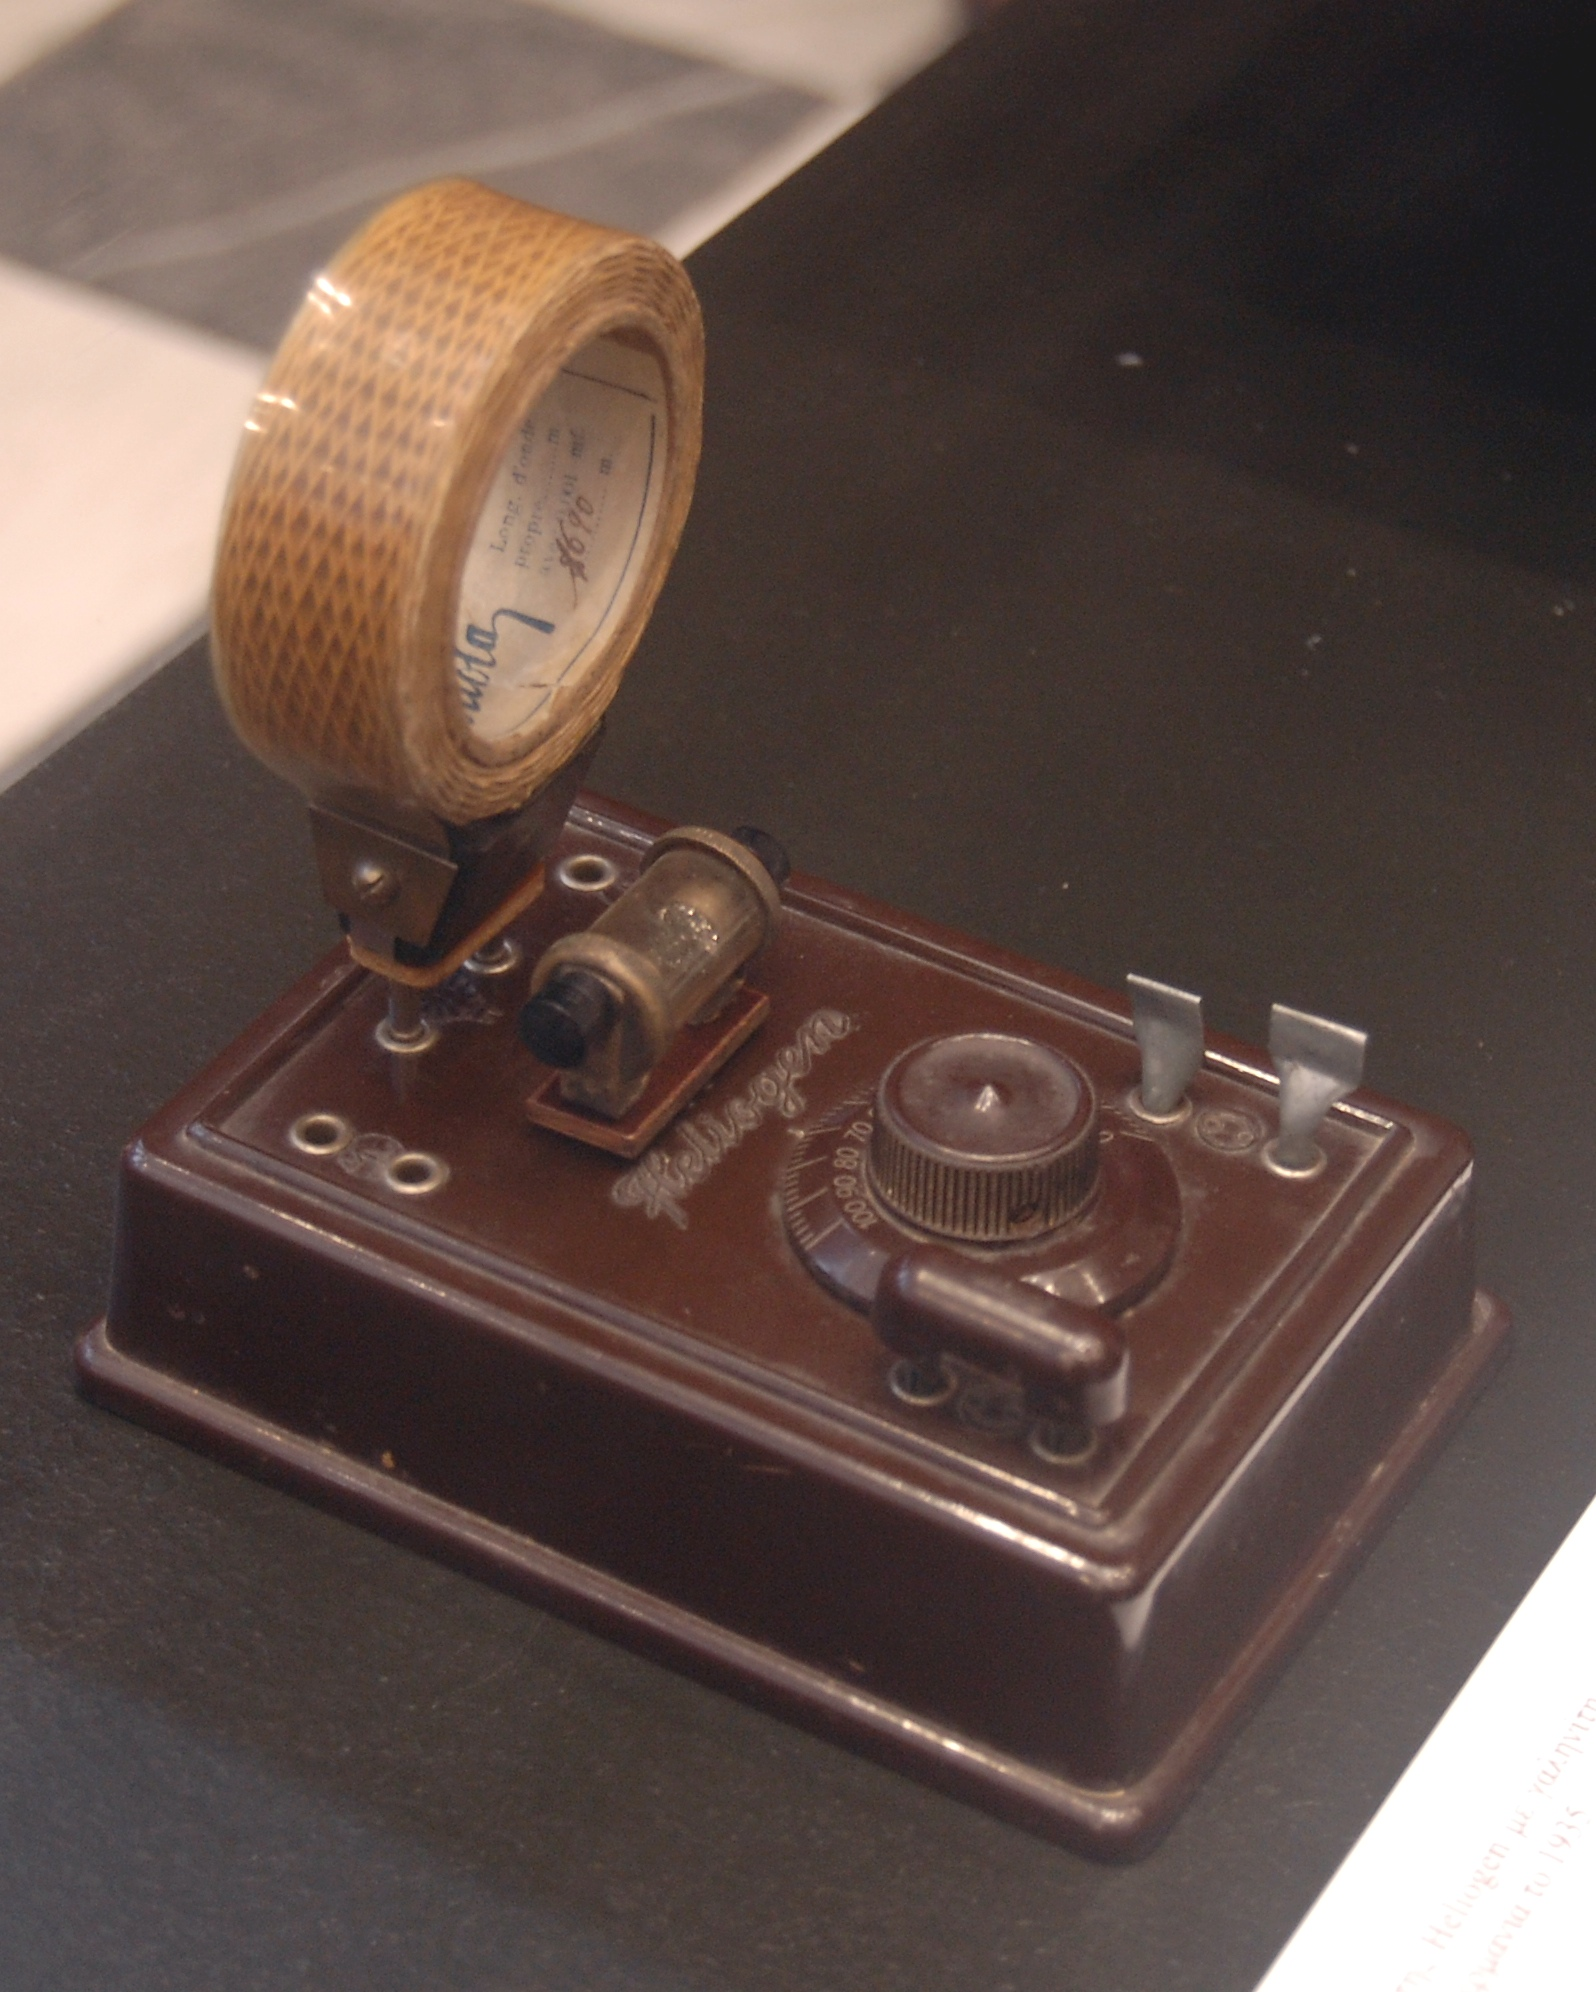
\includegraphics[scale=0.1]{Kurzwellendetektor/Bilder/Heliogen_medium_wave_galena_radio.JPG}
  %\caption{Historischer Detektorempfänger der Firma Heliogen (Deutschland 1935)}
 \vspace{-6cm}
\end{wrapfigure}

\section*{Praktische Anwendung}

\loesung{Mit den Lautsprechern funktioniert es ganz gut. Ggf. können sich die
SWL Kopfhörer mitbringen und diese mit einem Klinkenbuchsenadapter direkt
``anstöpseln.''

Mit der Spule um die $2.5 \mu H$ und dem DrehKo um die $200 pF$ befindet man
sich irgendwo im 40m-Band. Da Kurse meist Nachmittags/Abends stattfinden, bietet
sich dieses Band an. Für schnelle Erfolge kann man einen TRX mitnehmen und auf
dem Band in AM senden.

}

Radio- und Funk-Signale empfangen ohne die Verwendung einer Batterie oder einer
anderen Energiequelle? Eine einfache Schaltung ermöglicht das. Die folgende
Schaltung eines Detektorempfängers ist die einfachste aller Radioschaltungen. In
der Frühzeit der Radiotechnik war das Konzept eines Detektorempfänger durchaus
verbreitet. Heute ist es leider nich mehr ohne weiters möglich Radio-Sendungen
mit dem der Kurzwellendetektor zu empfangen, da der Großteil der Kurz- und
Mittelwellensender ihren Betrieb eingestellt haben. Nichts desto trotz ist er
ein guter Einstieg und ein technisches Abenteuer.

\begin{enumerate}
    %\itemsep1pt\parskip0pt\parsep0pt
    \item Baue die Schaltung aus Abbildung mit der bereits gebauten Spule
      \ref{kd} auf. Bei dem "`Detektor"' handelt es sich um eine Germaniumdiode
      (z.B. AA 143). Etwas weniger gut, aber weitaus preiswerter ist die
      Verwendung einer Schottky-Diode (z.B. BAT 43).  Was könnte die Diode tun
      und warum verwendet man keine Si-Dioden?
      \loesung{Dies ist ein Vorgriff auf die AM-Modulation. Die Diode
      demoduliert je nach Polung die obere oder untere Einhüllende.
      Germanium/Schottky-Dioden haben eine Schwellenspannung von ca. $0.3 V$,
      Silizium-Dioden arbeiten erst ab $0.6 V$ bis $0.7 V$.}
   \item Verwende den zuvor gebauten Audio-Verstärker, um empfangene Signale
     besser hörbar zu machen.
   \item Berechne den Schwingkreis. In welchem Band werden die Signale der
     Antenne empfangen? Verwendet ggf. das LC-Meter.  \loesung{Die SWL sollen
     das schön per Hand rechnen. Zum Nachprüfen kann man z.B. dieses Tool
     verwenden: http://wetec.vrok.de/rechner/cskreis.htm}
\end{enumerate}

\begin{figure}[H]
    \centering
    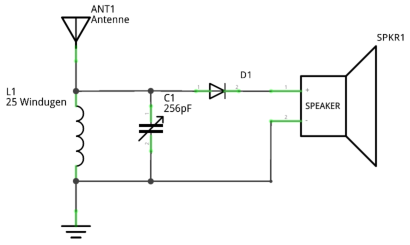
\includegraphics[scale=1]{Kurzwellendetektor/Bilder/Kurzwellendetektor_Schaltplan.pdf}
    \caption{Der Kurzwellendetektor}
    \label{kd}
\end{figure}
